%%%%%%%%%%%%%%%%%%%%%%%%%%%%%%%%%%%%%%%%%%%%%%%%%%%%%%%%%%%%%%%%%%%%%%
% How to use writeLaTeX: 
%
% You edit the source code here on the left, and the preview on the
% right shows you the result within a few seconds.
%
% Bookmark this page and share the URL with your co-authors. They can
% edit at the same time!
%
% You can upload figures, bibliographies, custom classes and
% styles using the files menu.
%
%%%%%%%%%%%%%%%%%%%%%%%%%%%%%%%%%%%%%%%%%%%%%%%%%%%%%%%%%%%%%%%%%%%%%%

\documentclass[12pt]{article}

\usepackage{sbc-template}

\usepackage{graphicx,url}

%\usepackage[brazil]{babel}   
\usepackage[utf8]{inputenc} 

\usepackage{float}
\usepackage{hyperref}
     
\sloppy

\title{Acionamento de Relé + Telegram}

\author{Fabricio Araújo Dias}

\address{Instituto Federal de Educação, Ciência e Tecnologia do Ceará
  (IFCE)\\
  Avenida Vice-Presidente José Alencar, S/N -- 61.939-140 -- Maracanaú -- CE -- Brasil
  \email{fabricio.araujo61@aluno.ifce.edu.br}
}

\begin{document} 

\maketitle

\begin{abstract}
  This report describes all the steps involved in carrying out the practical activity for the Microcontrollers course. The activity consists of using a relay to turn an LED on and off. The relay configuration is defined using commands from the bot created in the previous activity. It is necessary to configure the bot and handle the requests in the ESP32 code.
\end{abstract}
     
\begin{resumo} 
  Esse relatório descreve todos os passos para a realização da atividade prática da disciplina de Microcontroladores. A atividade consiste em utilizar um relé para acender e desligar um LED. Sendo que a configuração do relé é definida utilizando comandos do bot criado na aula. Se tornando necessário configurar o bot e tratar as requisições no código do ESP32.
\end{resumo}


\section{Introdução}\label{sec:introdução}
A quarta atividade prática consiste em acender e apagar um LED simples utilizando um relé. Isso utilizando novamente o bot do Telegram para mandar comando para o ESP32.

\section{Desenvolvimento do Código}\label{sec:desenvolvimento-do-código}

Primeiro, definimos a constante RELE 23 para representar o pino do ESP32 que irá conectar ao relé e enviar comandos. Em setup, configuramos o pino em modo de saída (OUTPUT) utilizando a função \textit{pinMode} e deixamos o pino em nível baixo (LOW) com a função \textit{digitalWrite}.

Em seguida, fazemos a configuração para conectar o ESP32 ao Wi-fi e ao bot do Telegram. Vamos para a página inicial do PlatformIO, acessamos a \textit{Libraries}, procuramos e instalamos a biblioteca \textit{Universal Telegram Bot}. Importamos as bibliotecas \textit{Wifi}, \textit{WifiClientSecure} e \textit{UniversalTelegramBot} no código. 

Definimos o SSID e a senha da rede Wi-fi, o token do bot do Telegram e o Chat Id. Instacionamos o client da classe \textit{WifiClientSecure} e o bot da classe \textit{UniversalTelegramBot} passando como parâmetros o token do bot e o client. 

Em setup, configuramos o módulo Wifi em \textit{station mode} para que ele conecte a um \textit{access point}, para então conectarmos à rede móvel do meu celular utilizando o método \textit{begin}. Conferindo se o Wi-fi foi conectado com sucesso utilizando o método \textit{status}, continuamos.

Antes de irmos para o loop, criamos uma função chamada \textit{handleNewMessages}, que vai pegar as mensagens do bot e alterar as configurações no ESP32. Ela recebe como parâmetros o número de mensagens do bot. A função possui um \textit{loop for} que itera até que a variável do laço chegue ao número de mensagem. A cada iteração, conferimos se o Chat Id do emissor da mensagem é o mesmo que definimos nas constantes, para evitar que alguém não autorizado utilize o bot. Descobrimos o Chat Id com \textit{bot.messages[i].chat\_id}.

Se o usuário está autorizado, guardamos o texto da mensagem e o nome do autor acessando os atributos \textit{text} e \textit{message}, respectivamente. O bot foi configurado com três comandos: start, led\_on e led\_off. Então, fizemos condicionais para cada um desses comandos. Se for start, o bot envia uma mensagem de boas vindas para o usuário e mostra os comandos que ele pode utilizar. Se for led\_on, manda uma mensagem dizendo que o LED está ligado e configura o pino do relé em nível alto. Se for led\_off, ele manda uma mensagem para o usuário dizendo que o LED está desligado e configura o pino do relé para nível baixo.

Indo para o loop, iremos utilizar o método getUpdates do bot para receber a quantidade de novas mensagens que ele recebeu. Passamos como parâmetro para esse método o índice da última mensagem recebida, acessando o atributo last\_message\_received, e somamos em 1 para termos o índice da primeira mensagem recebida e não lida. Guardando essa informações numa variável chamada numNewMessages, criamos um laço para que rode enquanto o valor de numNewMessages não seja 0, e nesse laço, nós chamamos a função handleNewMessage e passando a numNewMessages como parâmetro. Após, faremos o mesmo processo de chamar o método getUpdates do bot para atualizar a variável numNewMessages e conferir se não chegou outras mensagens.

Para finalizar, vamos estabelecer um delay no loop para que o número de requisições à API do Telegram seja absurda. Para isso, vamos definir uma constante DELAY de um 1000 ms e uma variável para guardar o tempo de execução do bot numa variável chamada de \textit{lastTimeBotRun}. Vamos utilizar a função millis da biblioteca do Arduino para descobrir o tempo em que o ESP32 está em execução. Colocamos, então, o que foi implementado dentro de um condicional if, e a condição é que só entra dentro do condicional se o tempo de execução atual for maior que a soma da variável lastTimeBotRun com o DELAY. \textit{LastTimeBotRun} é atualizada ao final do if, recebendo o valor de \textit{millis}.

É possível conferir o código nesse \href{https://github.com/fabricio-araujo94/microcontroladores/tree/main/acionamento_rele}{repositório no Github}.

\section{Configuração do Bot no Telegram}

O bot no Telegram precisa ser configurado para adicionar novos comandos e que ele envie para o ESP32. Acessando o \textit{BotFather} no Telegram, utilizamos o comando \textit{mybots} para que ele mostre os bots que criamos. Escolhemos o bot que criamos na aula passada, que é o \textit{algum123\_bot}. Pressionamos a opção \textit{Edit Bot}, e em seguida, pressionamos \textit{Edit Commands}. Adicionamos os comandos seguindo a sintaxe: comando - descrição do comando. Adicionando os comandos \textit{led\_on} e \textit{led\_off}, terminamos a configuração do bot.


\section{Configuração no ESP32}\label{sec:configuração-no-esp32}

Fizemos a conexão do pino 23 do ESP32 com o terminal \textit{INPUT 1} do relé. Para alimentar o relé, conectamos o terminal \textit{VCC} ao pino de \textit{VIN} que provê uma tensão de 5V que é o necessário para acionar o relé. O GND do relé é conectado ao GND do ESP32.

Garantindo a alimentação do relé, passamos a configurar a protoboard. O LED simples foi posicionado em um lugar qualquer com um resistor de 390 \textit{ohms} ligado ao seu terminal positivo. Para conectar o relé a protoboard, utilizamos dois cabos macho-macho para conectar os contatos do relé à protoboard. É necessário usar uma chave para abrir as entradas de contato do relé e, após conectado, fechá-la. Só foi necessário o contato comum e o contato normalmente aberto. Conectamos o contato comum à uma fonte de energia, e conectamos o contato normalmente aberto ao terminal positivo do LED através do resistor. O terminal negativo do LED é ligado à GND do ESP32.

\section{Considerações Finais}\label{sec:considerações-finais}\hfill

\begin{figure}[H]
    \centering
    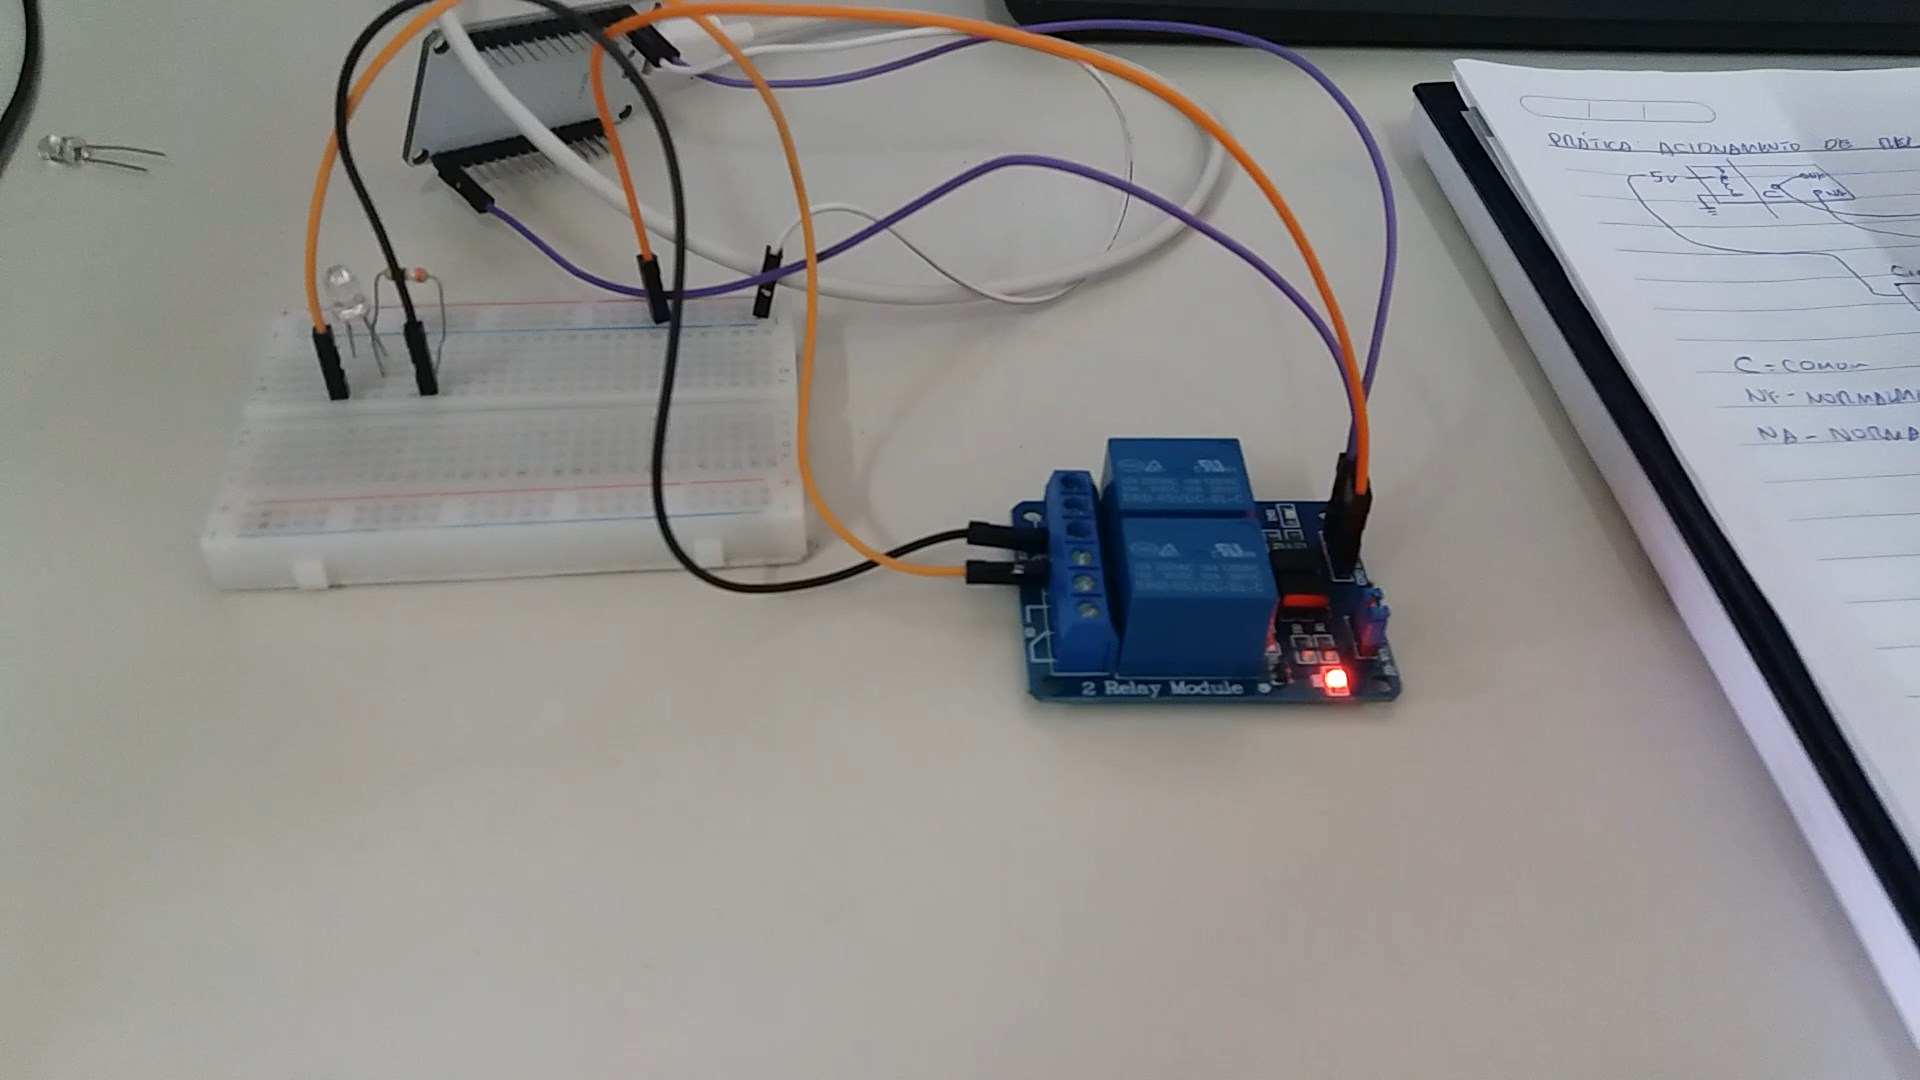
\includegraphics[width=0.5\linewidth]{img/20241106_100815.mp4_snapshot_00.06.067.jpg}
    \caption{Configuração na protoboard e no relé.}
    \label{fig:protoboard_relay}
\end{figure}

Conectando o ESP32 ao computador com o cabo microusb, enviamos o código que criamos para o microcontrolador. Agora, com os comandos, acendemos e apagamos o led cortando a corrente do relé utilizando comandos no bot do Telegram. Confira o \href{https://youtu.be/Syr4DVnW4ZM}{vídeo no Youtube} do resultado.

\end{document}
